%% SIGMETRICS 2027 / POMACS draft.
%% Format required by the CFP: \documentclass[acmsmall, screen, review]{acmart}
%% Up to 20 pages of technical content, single column; references unlimited.
%% Double-anonymous. Result cells are intentionally unfilled.
\documentclass[acmsmall,screen,review,anonymous]{acmart}

\usepackage{booktabs}
\usepackage{tabularx}
\usepackage{amsmath}
\usepackage{algorithm}
\usepackage{algpseudocode}
\usepackage{tikz}
\usetikzlibrary{arrows.meta,positioning,fit}

\newcommand{\systemname}{DynaByte}
\newcommand{\tbd}[1]{\textcolor{red}{[#1]}}
\newcommand{\PhiRatio}{\Phi}

\setcopyright{none}
\settopmatter{printfolios=true}
\renewcommand{\shortauthors}{Anonymous}

\acmJournal{POMACS}
\acmYear{2027}

\title{DynaByte: Allocating Expert Memory and Transfer Bandwidth for MoE Tail Latency}

%% Add the main end-to-end result and the gap to the strongest shared-budget
%% baseline after the joint evaluation is complete.
\begin{abstract}
How should a limited GPU allocate its expert memory and host-to-device transfer bandwidth among expert precision, residency, and lookahead, so that Mixture-of-Experts inference reduces tail latency under a quality-degradation limit?
Precision spends device bytes and increases the size of a later transfer, residency spends device bytes to avoid a transfer, and lookahead spends both bytes and bandwidth to hide a transfer that still occurs.
Existing policies usually fix two of these uses and optimize the third, so a precision quota or a prefetch depth tuned on its own can still raise tail latency once the two budgets are shared.
\systemname\ answers this question with donor-backed byte exchanges: each request names the precision, residency, or lookahead claim it displaces, and a deadline replay admits the exchange only when predicted exposed wait falls and the quality-degradation limit still holds.
One byte ledger and a publish-after-copy protocol keep the expert-memory peak within budget while the three uses are admitted together.
\end{abstract}

\begin{CCSXML}
<ccs2012>
<concept>
<concept_id>10010147.10010178</concept_id>
<concept_desc>Computing methodologies~Artificial intelligence</concept_desc>
<concept_significance>300</concept_significance>
</concept>
<concept>
<concept_id>10011007.10010940.10010941</concept_id>
<concept_desc>Software and its engineering~Memory management</concept_desc>
<concept_significance>500</concept_significance>
</concept>
<concept>
<concept_id>10010520.10010521</concept_id>
<concept_desc>Computer systems organization~Architectures</concept_desc>
<concept_significance>300</concept_significance>
</concept>
</ccs2012>
\end{CCSXML}

\ccsdesc[300]{Computing methodologies~Artificial intelligence}
\ccsdesc[500]{Software and its engineering~Memory management}
\ccsdesc[300]{Computer systems organization~Architectures}

\keywords{mixture of experts, memory management, prefetching, quantization, performance modeling}

\begin{document}

\maketitle

\noindent\textit{Draft status.}
This manuscript follows the SIGMETRICS~2027 \texttt{acmsmall} rules (at most 20 single-column pages of technical content, unlimited references, double-anonymous review).
Tables that depend on the joint re-measurement are marked in red and left blank.
The motivating measurements and trace replay in Sections~\ref{sec:obs-quality}--\ref{sec:obs-joint} are not end-to-end results for \systemname.

\section{Introduction}
\label{sec:intro}

A Mixture-of-Experts (MoE) layer routes each token to a small subset of expert subnetworks, allowing model capacity to grow without a proportional increase in per-token computation~\cite{shazeer2017outrageously,fedus2022switch,lepikhin2021gshard}.
The memory footprint remains large because every expert representation must still be stored or made available at inference time.
Models such as Mixtral, DeepSeek-V2, and Qwen3 contain tens to hundreds of billions of parameters while activating only a fraction of them for each token~\cite{jiang2024mixtral,deepseekv2,qwen3technicalreport}.
On a single accelerator, expert weights compete with non-expert parameters, the KV cache, activations, and runtime workspaces for device memory.
When experts cannot all remain at the desired precision, the system must both compress them and move them across the host-to-device link.

How should a limited GPU allocate its expert memory and host-to-device transfer bandwidth among expert precision, residency, and lookahead, so that Mixture-of-Experts inference reduces tail latency under a quality-degradation limit?

These two budgets meet in three uses.
Precision spends expert-memory bytes on a higher-precision representation and increases the size of any later transfer.
Residency spends bytes to keep an expert on the device so that a later access requires no transfer.
Lookahead spends both bytes and bandwidth to stage an absent expert early enough that an otherwise unavoidable transfer overlaps preceding computation.
A byte assigned to precision cannot also retain another expert or stage a future one.
Host-to-device bandwidth determines whether that early transfer finishes before its deadline.

Prior work has developed effective policies for parts of this problem.
Quantization and mixed-precision methods choose expert representations under a memory or accuracy target~\cite{lin2024awq,frantar2022gptq,duanmu2025mxmoe}.
Expert caches and prefetchers decide which experts to keep and when to transfer missing experts, commonly under a fixed representation size~\cite{song2024promoe,eliseev2023fast,xue2024moe,shen2025expertflow}.
Mixed-precision offloading systems demonstrate that lower-precision transfers, caching, and prefetching can coexist~\cite{tang2024hobbit,huang2026dymoe}.
The right assignment still changes with the workload: expert sensitivity sets the value of precision, routing locality sets the value of residency, and transfer deadlines set the value of lookahead.
A fixed partition or a fixed priority among the three uses cannot express these changing opportunity costs.
These systems show that the three mechanisms can operate together, yet they do not allocate expert memory and transfer bandwidth jointly among precision, residency, and lookahead under one quality-degradation limit.

\systemname\ answers this question.
Under a hard expert-memory budget \(B\) and a quality-degradation limit \(\epsilon\), it selects expert precision, residency, and prefetch timing to reduce tail latency.
The decision unit is a byte exchange: a requested expert state together with the precision, residency, or lookahead claim that would fund it.
Its value is the change in predicted exposed wait per requested byte after applying the complete exchange.
Quality risk is a feasibility constraint on that resulting state, rather than a latency reward.
\systemname\ represents each memory claim as a time-bounded \emph{byte lease} that records its owner, size, purpose, and expected lifetime.
A state monitor tracks routing demand, reuse, transfer deadlines, and quality-risk estimates.
It also measures \emph{in-overlap bandwidth}, the copy rate observed while expert computation is active.
A joint coordinator pairs requested leases with explicit \emph{donor leases}, the existing claims released to fund a request, and replays the deadline-ordered transfer queue before and after each exchange.
It admits only exchanges that improve predicted exposed wait while satisfying the quality-risk and peak-memory accounts.
Residency and lookahead refresh on a short time scale, and precision on a longer window, so that a precision change can amortize its migration cost.
Both rates use one admission path and the same byte ledger, which records published and reserved expert bytes. Neither rate receives a private quota.
The executor reserves memory before a copy begins, publishes a new expert representation only after the copy completes, and reclaims the old representation after its readers finish.

We make three contributions.
\begin{itemize}
  \item To answer this question, we formulate the joint allocation of expert memory and host-to-device transfer bandwidth among precision, residency, and lookahead. The objective is tail latency under a quality-degradation limit and a peak expert-memory budget. The formulation exposes opportunity costs hidden by independent precision, caching, and prefetch policies.
  \item We develop a byte-lease exchange policy that names the memory displaced by each request and counterfactually replays the resulting deadline schedule. Joint replay prevents residency and lookahead from receiving credit for the same avoided transfer and charges precision choices for their transfer cost.
  \item We design a runtime with one byte ledger and a publish-after-copy protocol. It admits transitions only when their peak footprint fits and never exposes an incomplete representation to the forward path.
\end{itemize}

% Upon acceptance, we will release the controller, runtime, routing-trace tools, and configurations for the reported experiments in a long-lived archive.

\section{Background and Motivation}
\label{sec:bg}

\subsection{Expert Bytes on One Accelerator}
\label{sec:serving}

An MoE layer \(\ell\) holds \(E_{\ell}\) routed experts and sends each token to \(k_{\ell}\) of them.
Expert weights are the movable object.
Non-expert parameters, the KV cache, activations, and a conversion workspace are sized for a declared maximum batch and sequence length and are reserved outside \(B\).
The runtime's allocation problem is only the expert budget.
Host memory holds a packed low-precision copy and a packed high-precision copy of each expert.
The device holds at most one live copy.
A live copy occupies either \(m^{\mathrm{lo}}_{\ell}\) or \(m^{\mathrm{hi}}_{\ell}\) bytes, both measured from the packed representation rather than from a nominal bit width.
Promoting an expert therefore costs \(m^{\mathrm{hi}}_{\ell}-m^{\mathrm{lo}}_{\ell}\) extra device bytes if a low-precision copy was already resident, and it costs \(m^{\mathrm{hi}}_{\ell}\) bytes if the expert was absent.

Three published mechanisms cover different corners of this state space.
Uniform post-training quantization assigns every expert the same bit width offline~\cite{frantar2022gptq,lin2024awq,dettmers2022gptint8,xiao2023smoothquant}.
The configuration is feasible only when the chosen width's pool fits in \(B\), and it cannot move fidelity when the router's hot set changes.
Cross-layer prefetch issues transfers for the experts predicted over the next \(S\) layers on a side stream, overlapping them with the compute of layers \(\ell,\ldots,\ell{+}S{-}1\)~\cite{song2024promoe,eliseev2023fast,hwang2024pre}.
\(S\) does not change routing.
It changes only how many distinct expert bytes the cache must absorb.
Mixed-precision offload uses a cheaper representation on the miss path so that a cache fill moves fewer bytes~\cite{tang2024hobbit,huang2026dymoe}.
The bit width in that design is a property of the transfer, not a pin that is protected from eviction.

\subsection{Preliminary Measurements}
\label{sec:prelim}

The joint protocol in Section~\ref{sec:eval} repeats the following measurements on one runtime.
We report them here because they fix the quantities the model has to explain.
All three were taken on an NVIDIA RTX~A6000~\cite{nvidiaA6000datasheet}.
They are not comparable to each other as end-to-end system results: the density and hot-set traces use the model's native routing with experts forced to the low tier, and the horizon sweep uses a separate 20\,GB residency cap.

\paragraph{Activation density swings inside one request.}
We define the unique-expert ratio of a step as the number of distinct experts selected by top-\(k\) routing, divided by \(E_{\ell}\), averaged over routed layers.
The average is over five fixed prompt blocks.
Batch \(b\) uses the first \(b\) prompts of a 32-prompt block.
Prefill is the unique set over all non-padding tokens of a prompt capped at 2{,}048 tokens.
Decode is the unique set of the single next token, not an accumulation over a long generation.
Table~\ref{tab:density} shows the ratio on three models.
On Qwen3-30B at batch 32 the prefill ratio is 94.0\% and the next decode step is 26.0\%.
On Phi-3.5-MoE the prefill ratio is essentially the entire pool at every batch we measured.
A horizon chosen for the decode working set does not describe the prefill working set of the same request.

\begin{table}[t]
  \centering
  \caption{Preliminary unique-expert activation ratio (\%), RTX~A6000.
  Each cell averages routed layers and five prompt blocks.
  Prefill accumulates the prompt; decode is one subsequent token.
  The joint protocol repeats this table before any system comparison.}
  \label{tab:density}
  \small
  \begin{tabular}{@{}llrrrrrr@{}}
    \toprule
    Model & Stage & 1 & 2 & 4 & 8 & 16 & 32 \\
    \midrule
    Qwen3-30B & Decode & 6.3 & 7.9 & 11.8 & 16.1 & 20.8 & 26.0 \\
              & Prefill & 59.8 & 70.0 & 82.9 & 89.7 & 92.4 & 94.0 \\
    Qwen3-Next-80B & Decode & 1.9 & 3.7 & 6.7 & 14.9 & 25.4 & 39.2 \\
                   & Prefill & 24.6 & 35.3 & 48.8 & 67.1 & 78.9 & 86.2 \\
    Phi-3.5-MoE & Decode & 12.5 & 22.7 & 37.1 & 59.3 & 77.8 & 88.8 \\
                & Prefill & 98.2 & 98.8 & 99.4 & 99.8 & 99.9 & 100.0 \\
    \bottomrule
  \end{tabular}
\end{table}

\paragraph{The hot set is a property of the task.}
On Qwen3-30B, Layer~15, we counted every selected top-\(k\) dispatch under three full workloads (WikiText, GSM8K, and HumanEval) with the scheduler frozen and every expert held at low precision.
The ten most frequently selected experts were disjoint across the three workloads.
A high-precision assignment computed on one calibration corpus therefore pins the wrong experts on the other two tasks.
The slow loop has to be allowed to change identities.
It also has to be slow: a swap replaces a resident block and consumes migration bandwidth.

\paragraph{The horizon has a U-shaped latency curve when the pool does not fit.}
Under a 20\,GB device cap that forces expert absence, latency against \(S\) on three smaller MoE models was U-shaped.
Below the minimum, transfers do not finish inside the compute of the next \(S\) layers and the critical path accumulates exposed wait.
Above the minimum, the speculative set exceeds the cap, evictions increase, and later misses reload experts that a smaller horizon would have kept.
The location of the minimum differed by model on the same device.
Holding \(S\) fixed and increasing the batch from 1 to 32 increased the waiting component by up to \(2.5\times\).
At fixed batch size, requests with higher intra-batch embedding dispersion activated more distinct experts and showed up to \(300\%\) end-to-end latency variation against low-dispersion requests of the same length.
Effective host-to-device bandwidth across the devices used in that sweep spans roughly an order of magnitude, from a low-bandwidth discrete GPU to NVIDIA~H20 and Ascend~910B at about 128\,GB/s.
A horizon selected on one (device, batch, dispersion) triple is a different point on the curve for the others.

These three facts are the constraints on the model.
Density determines how many distinct experts a step demands.
Task identity determines which of those experts are worth a high-precision pin, on a slower timescale than a single layer.
Bandwidth, batch, and dispersion move the horizon that hides transfers, and they do so only when absence is unavoidable.
The rest of this section writes those constraints as a budget ratio and an overlap predicate.

\subsection{The Budget Ratio}
\label{sec:model}

Let \(P_{\mathrm{lo}}=\sum_{\ell} E_{\ell}\, m^{\mathrm{lo}}_{\ell}\) and \(P_{\mathrm{hi}}=\sum_{\ell} E_{\ell}\, m^{\mathrm{hi}}_{\ell}\).
Both sums are known once the packed representations have been materialized.
The deployment ratio is \(\PhiRatio=B/P_{\mathrm{lo}}\).
Staging for a publish-before-reclaim overlap is a constant \(M_{\mathrm{stage}}=K \max_{\ell,b} m^{b}_{\ell}\), with \(K\) the maximum number of in-flight transitions.
The controller spends \(B-M_{\mathrm{stage}}\).
We fold \(M_{\mathrm{stage}}\) into the definition of the usable budget from here on and continue to call it \(B\), so the inequalities below are stated against the usable budget.
Figure~\ref{fig:phase} is a schematic of the resulting regimes, not a measurement.

\begin{figure}[t]
  \centering
  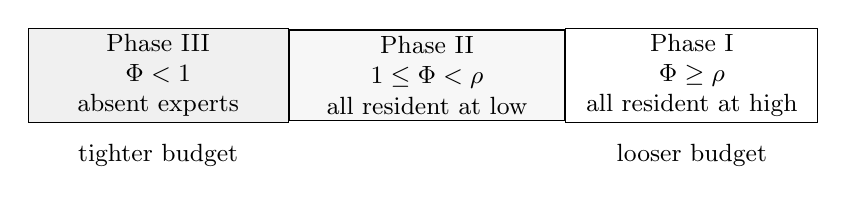
\begin{tikzpicture}[
      font=\small,
      box/.style={draw, minimum height=1.15cm, inner sep=2pt, align=center},
      arr/.style={-{Stealth}, thick}
    ]
    \node[box, minimum width=3.3cm, fill=black!6] (p3) {Phase III\\ \(\PhiRatio<1\)\\ absent experts};
    \node[box, minimum width=3.5cm, fill=black!3, right=0pt of p3] (p2) {Phase II\\ \(1\le\PhiRatio<\rho\)\\ all resident at low};
    \node[box, minimum width=3.2cm, fill=white, right=0pt of p2] (p1) {Phase I\\ \(\PhiRatio\ge\rho\)\\ all resident at high};
    \node[below=0.15cm of p3, align=center] {tighter budget};
    \node[below=0.15cm of p1, align=center] {looser budget};
  \end{tikzpicture}
  \Description{Three adjacent boxes labeled Phase III, Phase II, and Phase I, ordered from a tighter budget to a looser budget.}
  \caption{Regimes of the expert-byte budget.
  \(\rho=P_{\mathrm{hi}}/P_{\mathrm{lo}}\).
  Phase~II spends leftover bytes on high-precision pins and sets the horizon to zero.
  Phase~III spends bytes first on the smallest feasible horizon, then on pins.
  The figure is the model's partition; Section~\ref{sec:eval} checks it against measured latency.}
  \label{fig:phase}
\end{figure}

\paragraph{Phase I.}
If \(B \ge P_{\mathrm{hi}}\), every expert fits at high precision.
The latency and quality costs of migration are both zero at the all-high assignment.
\systemname\ loads that assignment and disables both loops.

\paragraph{Phase II.}
If \(P_{\mathrm{lo}} \le B < P_{\mathrm{hi}}\), every expert fits at low precision and the all-high assignment does not fit.
Absence is unnecessary.
Any prefetch that moves an expert already resident adds a transfer and does not remove one.
The horizon that minimizes transfer latency is therefore \(S^{\star}=0\).
Replacing a low-precision resident with a high-precision resident costs \(m^{\mathrm{hi}}_{\ell}-m^{\mathrm{lo}}_{\ell}\) additional bytes.
When expert sizes are uniform within a layer and the same across layers, the maximum number of high-precision experts per layer satisfies
\begin{equation}
  n_{\mathrm{hi}}
  \;\le\;
  \left\lfloor
    \frac{B-P_{\mathrm{lo}}}{m^{\mathrm{hi}}-m^{\mathrm{lo}}}
    \cdot
    \frac{1}{L}
  \right\rfloor,
  \label{eq:phase2-nhi}
\end{equation}
with \(L\) the number of MoE layers, the floor applying after a proportional split.
The general case without that uniformity assumption is the integer knapsack that maximizes \(\sum_{\ell} n_{\mathrm{hi},\ell}\) subject to \(\sum_{\ell} n_{\mathrm{hi},\ell}(m^{\mathrm{hi}}_{\ell}-m^{\mathrm{lo}}_{\ell}) \le B-P_{\mathrm{lo}}\) and \(0 \le n_{\mathrm{hi},\ell} \le E_{\ell}\).
We use the proportional split in the implementation and record the knapsack as an optimality gap to measure, not as the online algorithm.
Identities inside the quota are the only online decision in this phase.
They are ranked by the slow hotness score of Section~\ref{sec:slow}.

As a numerical illustration of the algebra, not as a measured operating point: if \(m^{\mathrm{hi}}=4\,m^{\mathrm{lo}}\) and \(B=1.5\,P_{\mathrm{lo}}\), then \(\PhiRatio=1.5\) and the high-precision share of the pool is \((\PhiRatio-1)/(\rho-1)=1/6\).
About one sixth of the experts can be pinned high, and the rest stay resident at low precision.
A horizon controller that still evicts cold experts to ``make room'' destroys the floor that made \(S^{\star}=0\) feasible.

\paragraph{Phase III.}
If \(B < P_{\mathrm{lo}}\), a complete low-precision floor does not fit.
Some experts are absent, and a miss moves \(m\) bytes, where \(m\) is the size of the representation being fetched.
Let \(\hat{U}(S)\) be the set of experts the predictor expects to touch over the next \(S\) MoE layers, and let \(R\) be the set currently resident.
The miss set is \(\hat{U}(S)\setminus R\), and its transfer size is
\begin{equation}
  M_{\mathrm{miss}}(S)
  \;=\;
  \sum_{(\ell,e)\in \hat{U}(S)\setminus R} m_{\ell,e},
  \label{eq:miss-bytes}
\end{equation}
where \(m_{\ell,e}\) equals \(m^{\mathrm{hi}}_{\ell}\) if \((\ell,e)\) is a high-precision pin and \(m^{\mathrm{lo}}_{\ell}\) otherwise.
Pins are not misses.
A horizon \(S\) hides that transfer when two predicates hold simultaneously:
\begin{align}
  M_{\mathrm{miss}}(S) &\;\le\; S \cdot T_{\ell} \cdot C,
  \label{eq:overlap}\\
  \mathrm{bytes}(R \cup \hat{U}(S)) &\;\le\; B.
  \label{eq:fit}
\end{align}
Equation~\eqref{eq:overlap} is the overlap window.
Equation~\eqref{eq:fit} is cache pollution written as a hard constraint: a horizon whose speculative set does not fit is not a candidate, rather than a candidate with a penalty weight.
Define
\begin{equation}
  S^{\star}
  \;=\;
  \min\{\, S \in [S_{\min}, S_{\max}] : \eqref{eq:overlap}\ \mathrm{and}\ \eqref{eq:fit}\,\},
  \label{eq:sstar}
\end{equation}
and call the feasible set empty when no such \(S\) exists.
The minimum is the latency-optimal choice under a lexicographic rule: meet the overlap constraint, then leave the largest possible slack \(B-\mathrm{bytes}(R \cup \hat{U}(S^{\star}))\) for high-precision pins.
A larger feasible horizon would also hide the mean transfer and would consume bytes that could have raised \(n_{\mathrm{hi}}\).

The empty-set case is the dense sub-phase.
It is what Table~\ref{tab:density} suggests during prefill at high batch: \(\hat{U}(S)\) grows toward the full pool, \(M_{\mathrm{miss}}(S)\) exceeds both the overlap window and \(B\), and increasing \(S\) makes~\eqref{eq:fit} fail sooner.
The latency-minimizing action is then \(S^{\star}=S_{\min}\), with resident slots filled by the immediate layer's demand and then by the slow hotness order.
The non-empty case is the sparse sub-phase, typical of a small decode working set.
There \(S^{\star}\) is achievable, and every byte above \(\mathrm{bytes}(\hat{U}(S^{\star}))\) is slack.

Tail demand uses the same predicate.
Let \(M^{\mathrm{p95}}_{\mathrm{miss}}(S)\) be~\eqref{eq:miss-bytes} evaluated at the 95th percentile of the miss-set size observed over a sliding window of recent batches at this layer, with expert size \(m^{\mathrm{lo}}\) for unpinned experts.
The controller substitutes \(M^{\mathrm{p95}}_{\mathrm{miss}}\) for \(M_{\mathrm{miss}}\) in~\eqref{eq:overlap}.
The mean-demand horizon remains the quantity we plot against the model; the percentile horizon is what the runtime tracks.
Section~\ref{sec:eval} reports both, because a model that predicts the mean and misses the tail has not met a latency objective.

\subsection{What the Model Predicts}
\label{sec:predictions}

The regime rules are predictions about latency, not about task score.
Quality enters only as the use of slack.
We separate them so that a failure of the hotness proxy does not get mistaken for a failure of the overlap identity.

\begin{description}
  \item[P1.] In Phase~II the horizon that minimizes exposed expert-transfer latency is \(S=0\). A positive horizon increases migration bytes and does not reduce misses.
  \item[P2.] In Phase~III, when the feasible set is non-empty, \(S^{\star}\) is non-increasing in \(C\) and non-decreasing in the byte size \(m\) of a prefetched expert. Replacing a low-precision prefetch with a high-precision prefetch shifts \(S^{\star}\) up or empties the feasible set.
  \item[P3.] At fixed \(\PhiRatio<1\), a request can move from an empty feasible set during prefill to a non-empty set during decode. The minimizing action changes from ``fill the immediate resident set, hold \(S\) at \(S_{\min}\)'' to ``track \(S^{\star}\), then pin from the slack.''
  \item[P4.] Under the lexicographic rule, \(n_{\mathrm{hi}}\) is bounded by the slack after \(S^{\star}\) has been reserved. Raising \(S^{\star}\), raising \(m^{\mathrm{hi}}\), or entering the dense sub-phase all shrink that bound, including down to zero.
\end{description}

P1--P4 are the claims a joint re-measurement has to accept or reject.
They also state the boundary policies precisely.
A precision-only policy is the Phase~II optimum, including its \(n_{\mathrm{hi}}\) bound, applied at every \(\PhiRatio\).
When \(\PhiRatio<1\) that policy has no feasible full floor; an implementation must either exceed \(B\) or silently fall back to a tighter quantization.
A horizon-only policy is the Phase~III rule with \(m\) fixed and \(n_{\mathrm{hi}}\) fixed at zero, applied at every \(\PhiRatio\).
When \(\PhiRatio\ge 1\) it evicts experts the budget could have kept.
A naive composition runs both controllers and lets each assume it may use \(B\).
The composition violates~\eqref{eq:fit} whenever the pin quota and the speculative set are computed independently.
Section~\ref{sec:design} is the tracker that enforces one budget across both timescales.
Section~\ref{sec:eval} measures the four predictions before it measures that tracker against the boundary policies.

\subsection{Inputs the Model Does Not Observe}
\label{sec:model-limits}

The overlap identity uses a scalar \(C\).
Concurrent compute traffic reduces the bandwidth that a side-stream copy actually receives.
\systemname\ estimates \(C\) from completed transfers during overlap, not from an idle bandwidth benchmark, and Section~\ref{sec:eval} reports the error of \(S^{\star}\) under both estimators.
Dequantization and the launch of a second grouped GEMM, one per live precision in the layer, add device time that is not a host-to-device transfer.
Those times sit inside the measured \(T_{\ell}\).
They shrink the overlap window rather than appearing as a separate miss term.
The model does not predict task score.
Hotness is a proxy for which expert should receive a slack byte, and it can be wrong while P1--P3 still hold.
Kernel-launch overhead and proxy error are measured quantities in Section~\ref{sec:eval}, not terms hidden inside \(\PhiRatio\).

\section{Design}
\label{sec:design}

\subsection{Overview}
\label{sec:model}

\systemname\ answers the allocation question with one admission procedure.
It represents a change of precision, residency, or lookahead as a donor-backed byte exchange, scores that exchange by the predicted exposed wait it saves per byte, and admits it only while the quality-risk account and the expert-memory ledger both hold.
One executor then commits the admitted schedule.
Host-to-device bandwidth has no separate quota: the deadline replay charges each exchange for the migration-queue time its transfers occupy.

The procedure has five steps.
\begin{enumerate}
  \item Observe one snapshot of routing demand, quality risk, deadlines, bandwidth, and byte state.
  \item Generate candidate leases for fidelity, residency, and lookahead inside one candidate envelope.
  \item Attach donor leases to each request and score the complete exchange with one deadline replay.
  \item Admit exchanges in decreasing saved wait per byte while both accounts remain feasible.
  \item Commit each admitted exchange by reserving, copying, publishing, and reclaiming on one arena.
\end{enumerate}
The four components in the rest of this section implement these steps.
None of them optimizes tail latency on its own.

Every precision, retention, and prefetch decision is the exchange
\begin{equation}
  x=(Z^{+},D,\mathcal{T}),
  \label{eq:exchange}
\end{equation}
where \(Z^{+}\) is the compatible set of leases to create or renew, \(D\) is the set of leases released to fund them, and \(\mathcal{T}\) is the transition schedule during which old and new representations may coexist.
The coordinator evaluates the state after the whole exchange, so the value of one use includes its effect on the other two.
Quality risk and peak bytes are feasibility checks on that state.
A shared ledger reserves the complete schedule \(\mathcal{T}\), so concurrent exchanges cannot spend the same released bytes.

\paragraph{Optimization contract.}
Let a runtime policy \(\pi\) choose the representation, resident set, and transfer issue time of every expert.
Expert memory enters as the hard budget \(B\).
Host-to-device bandwidth is the measured rate of the migration queue replayed below, the same rate defined in Section~\ref{sec:serving}.
The objective constrains expert memory and quality; bandwidth is accounted for inside that replayed schedule.
\begin{equation}
  \min_{\pi}\; \operatorname{P95}(\mathrm{TPOT};\pi)
  \quad \text{subject to} \quad
  M_{\mathrm{peak}}(\pi) \le B,
  \qquad
  \Delta Q(\pi) \le \epsilon.
  \label{eq:objective}
\end{equation}
Background reserves non-expert weights, the KV cache, activations, and fixed workspaces before deriving \(B\).
The quality-degradation limit is measured against a fixed reference configuration for each task.
The runtime uses a calibrated risk estimate to guide decisions; Section~\ref{sec:quality-boundary} states why that estimate is not a per-request quality guarantee.

An expert \(i=(\ell,e)\) is absent, resident at low precision, resident at high precision, or in transition toward one of the resident states.
Let its packed footprints be \(m_i^{\mathrm{lo}}\) and \(m_i^{\mathrm{hi}}\).
A high-precision resident consumes a low-precision residency footprint plus the fidelity increment
\begin{equation}
  \delta m_i^{\mathrm{fid}}
  =m_i^{\mathrm{hi}}-m_i^{\mathrm{lo}}.
  \label{eq:fidelity-increment}
\end{equation}
The decomposition is logical; a high-precision representation remains one packed block.
Only a published resident representation is executable.
A destination under transfer is reserved but not published, and an old representation with outstanding readers remains published until reclamation.

\paragraph{One exchange, end to end.}
Consider an absent expert predicted two layers ahead when no free block remains.
The snapshot records the expert as absent, names its deadline, and reports that the byte ledger has no slack.
The generator emits a lookahead lease for the selected representation.
The coordinator pairs that request with the resident it would evict and, when more bytes are required, with the fidelity increment it would release.
One replay compares predicted exposed wait before and after the exchange.
Admission requires the saved wait to exceed the donor's future miss and migration cost, the provisional quality-risk account to hold, and the peak footprint of the transition to fit \(B\).
The executor then reserves the destination, copies into it, publishes the new representation, and reclaims the donor after its readers finish.
The same five steps apply when the request is a fidelity upgrade or a residency renewal; only the donor and the term changed in the replay differ.

Figure~\ref{fig:arch} assigns the steps to four components.
The state monitor builds the snapshot in step~1.
The lease generator and valuator produce the candidate leases in step~2 and compute the score used in step~3.
The exchange coordinator attaches donors and performs the admission in step~4.
The safe executor commits the schedule in step~5.

\begin{figure}[t]
  \centering
  % Editable TikZ source for the DynaByte design overview.
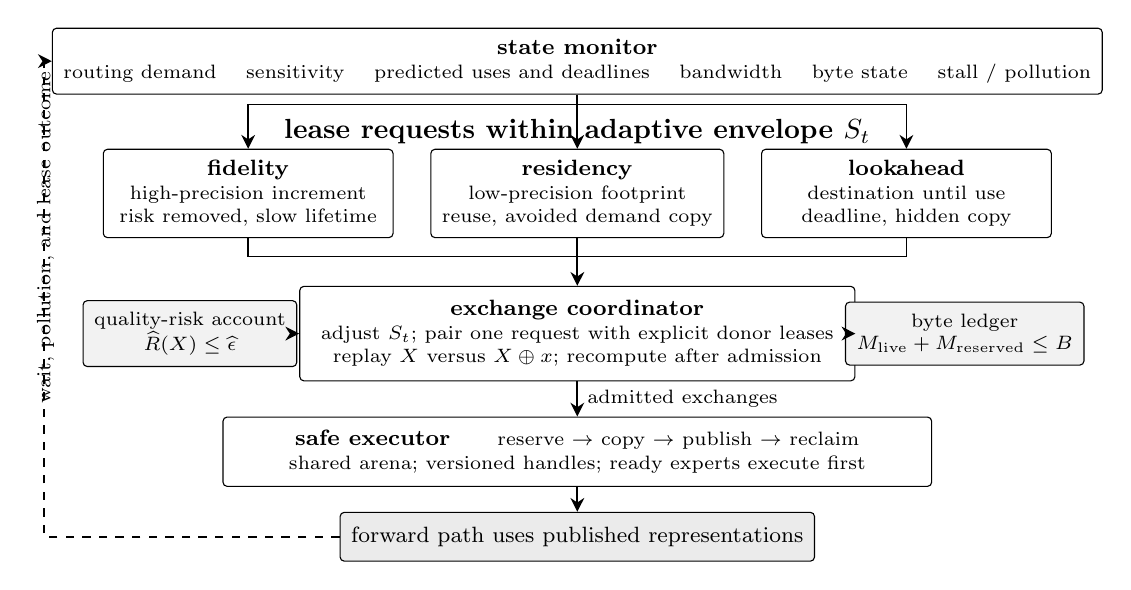
\begin{tikzpicture}[
    font=\footnotesize,
    >=Stealth,
    flow/.style={-{Stealth[length=5pt,width=5pt]}, semithick},
    feedback/.style={-{Stealth[length=5pt,width=5pt]}, semithick, dashed},
    block/.style={draw, rounded corners=1.5pt, align=center, inner sep=4pt},
    lease/.style={block, minimum width=3.68cm, minimum height=1.02cm},
    account/.style={block, minimum width=2.62cm, minimum height=0.80cm,
                    fill=black!5, font=\scriptsize}
  ]

  \node[block, minimum width=12.6cm, minimum height=0.78cm] (monitor) at (0,0)
    {\textbf{state monitor}\\[-1pt]
     \scriptsize routing demand \quad sensitivity \quad predicted uses and deadlines
     \quad bandwidth \quad byte state \quad stall / pollution};

  \node[font=\bfseries, fill=white, inner sep=1.5pt] at (0,-0.90)
    {lease requests within adaptive envelope \(S_t\)};
  \node[lease] (fidelity) at (-4.18,-1.68)
    {\textbf{fidelity}\\[-1pt]
     \scriptsize high-precision increment\\[-1pt]
     \scriptsize risk removed, slow lifetime};
  \node[lease] (residency) at (0,-1.68)
    {\textbf{residency}\\[-1pt]
     \scriptsize low-precision footprint\\[-1pt]
     \scriptsize reuse, avoided demand copy};
  \node[lease] (lookahead) at (4.18,-1.68)
    {\textbf{lookahead}\\[-1pt]
     \scriptsize destination until use\\[-1pt]
     \scriptsize deadline, hidden copy};

  \coordinate (fanout) at (0,-0.55);
  \draw[flow] (monitor.south) -- (fanout) -| (fidelity.north);
  \draw[flow] (fanout) -- (residency.north);
  \draw[flow] (fanout) -| (lookahead.north);

  \node[block, minimum width=7.05cm, minimum height=1.20cm] (coord) at (0,-3.46)
    {\textbf{exchange coordinator}\\[-1pt]
     \scriptsize adjust \(S_t\); pair one request with explicit donor leases\\[-1pt]
     \scriptsize replay \(X\) versus \(X\oplus x\); recompute after admission};
  \node[account] (quality) at (-4.92,-3.46)
    {quality-risk account\\\(\widehat R(X)\leq\widehat\epsilon\)};
  \node[account] (ledger) at (4.92,-3.46)
    {byte ledger\\\(M_{\mathrm{live}}+M_{\mathrm{reserved}}\leq B\)};

  \coordinate (fanin) at (0,-2.48);
  \draw[semithick] (fidelity.south) |- (fanin);
  \draw[semithick] (residency.south) -- (fanin);
  \draw[semithick] (lookahead.south) |- (fanin);
  \draw[flow] (fanin) -- (coord.north);
  \draw[flow] (quality) -- (coord);
  \draw[flow] (ledger) -- (coord);

  \node[block, minimum width=9.0cm, minimum height=0.88cm] (executor) at (0,-4.96)
    {\textbf{safe executor}\qquad
     \scriptsize reserve \(\rightarrow\) copy \(\rightarrow\) publish \(\rightarrow\) reclaim\\[-1pt]
     \scriptsize shared arena; versioned handles; ready experts execute first};
  \node[block, minimum width=4.9cm, minimum height=0.62cm, fill=black!8]
    (forward) at (0,-6.04)
    {forward path uses published representations};

  \draw[flow] (coord) -- node[right, font=\scriptsize] {admitted exchanges} (executor);
  \draw[flow] (executor) -- (forward);
  \draw[feedback] (forward.west) -- ++(-3.75,0) |-
    node[pos=0.58, left, rotate=90, font=\scriptsize] {wait, pollution, and lease outcome}
    (monitor.west);
\end{tikzpicture}

  \Description{DynaByte observes routing demand, offline sensitivity, predicted uses and deadlines, in-overlap bandwidth, published plus reserved bytes, and recent stall and pollution. Fidelity, residency, and lookahead leases are inputs to one exchange coordinator. The coordinator pairs a request with explicit donor leases, replays the predicted transfer queue before and after the exchange, and checks the quality-risk and byte accounts. A safe executor uses a shared arena and versioned handles to reserve, copy, publish, and reclaim admitted exchanges. Execution outcomes feed back into the monitor.}
  \caption{\systemname\ runs one admission procedure.
  The state monitor builds the snapshot (step~1).
  Fidelity, residency, and lookahead leases are inputs to one exchange coordinator, which scores each complete exchange and admits it (steps~2--4).
  The safe executor commits the admitted schedule (step~5).}
  \label{fig:arch}
\end{figure}

Table~\ref{tab:lease-transitions} is the action space of step~2.
Low- and high-precision loads of an absent expert are mutually exclusive candidates.
A high-precision load occupies one physical block, although its resident state is accounted logically as a base residency lease plus a fidelity increment.

\begin{table}[t]
  \caption{Lease transitions in the common action space. ``Release'' occurs only after the transition in the last column makes the bytes reclaimable.}
  \label{tab:lease-transitions}
  \small
  \setlength{\tabcolsep}{3pt}
  \begin{tabularx}{\columnwidth}{@{}>{\raggedright\arraybackslash}p{0.17\columnwidth}>{\raggedright\arraybackslash}p{0.19\columnwidth}>{\raggedright\arraybackslash}X>{\raggedright\arraybackslash}p{0.22\columnwidth}@{}}
    \toprule
    Current & Requested & Lease change & Transition \\
    \midrule
    absent & in flight (low/high) & acquire lookahead of \(m_i^{\mathrm{lo}}\) or \(m_i^{\mathrm{hi}}\) & reserve, copy \\
    resident (low) & resident (high) & acquire fidelity of \(\delta m_i^{\mathrm{fid}}\) & promote, publish \\
    resident (high) & resident (low) & release fidelity & demote, publish \\
    resident (low/high) & absent & release residency and any fidelity & drain readers, reclaim \\
    lookahead & resident (same tier) & convert lookahead into residency and any fidelity & publish, reclassify \\
    \bottomrule
  \end{tabularx}
\end{table}

\subsection{State Monitor}
\label{sec:monitor}

The state monitor's only output is the snapshot consumed by step~1.
It selects no exchange and promotes no expert.

For each expert, it distinguishes the published state used by dispatch, a reserved transition accepted by the executor, and the provisional state considered by the coordinator.
It also records recent uses, predicted next-use time, and the device location of every published or reserved representation.
Per-layer counters record expert-kernel time, in-overlap bandwidth, and exposed wait attributed to missing experts.
The monitor reports published and reserved bytes separately.
A provisional state consumes no capacity until admission.
A destination bound by a reserved transition does.

Two measurements tell the coordinator whether the candidate envelope should grow or shrink.
The stall signal \(s_t\) is the fraction of routed-layer time exposed while waiting for expert transfers during fast period \(t\).
We define \emph{lookahead pollution} \(p_t\) as the sum of unused lookahead bytes and bytes reloaded after a speculative displacement, divided by \(\max(B_t^{\mathrm{look}},b_{\min})\).
Here \(B_t^{\mathrm{look}}\) is the lookahead traffic admitted in the period and \(b_{\min}\) is the smallest packed expert block.
The monitor smooths both signals:
\begin{equation}
  \widetilde s_t=\beta\widetilde s_{t-1}+(1-\beta)s_t,
  \qquad
  \widetilde p_t=\beta\widetilde p_{t-1}+(1-\beta)p_t.
  \label{eq:lookahead-feedback}
\end{equation}
Stall indicates that the envelope may be too short; pollution indicates that looking farther ahead is consuming bytes without hiding useful work.
Keeping the two measurements separate distinguishes a late correct prediction from an early false positive.
Section~\ref{sec:coordinator} applies them; the monitor does not update the envelope.

The quality-risk estimate separates the harm of an expert's low representation from the frequency with which that representation is expected to execute.
An offline sensitivity \(q_i\geq 0\) measures the nonnegative increase in calibration loss when only expert \(i\) uses the low representation.
The runtime does not modify \(q_i\).
After a forward step with \(N_{\ell}\) routed positions, it measures expert \(e\)'s routing demand as
\begin{equation}
  c_{\ell,e}
  =
  \frac{1}{N_{\ell}}
  \sum_{t=1}^{N_{\ell}}
  \mathbf{1}[e\in\mathcal{R}_{\ell,t}]\,p_{\ell,t,e},
  \label{eq:hotness}
\end{equation}
where \(p_{\ell,t,e}\) is the router weight.
The monitor applies \(w_i\leftarrow\alpha w_i+(1-\alpha)c_i\).
The quantity \(w_i\) is a routing weight, not a quality score.

For a planned state \(X\), let \(h_i(X)=1\) when expert \(i\)'s next execution uses the high representation and zero otherwise.
The monitor computes
\begin{equation}
  \widehat R(X)
  =\sum_i w_i q_i\bigl(1-h_i(X)\bigr).
  \label{eq:risk}
\end{equation}
A proxy limit \(\widehat\epsilon\) is chosen on the calibration split together with the actual quality-degradation limit \(\epsilon\).
The coordinator uses \(\widehat R(X)\le\widehat\epsilon\) as a feasibility check and never converts risk into milliseconds.

The same snapshot stores recent routing transitions and, when available, pre-gating (pregate) logits emitted before the target MoE layer.
The generator in Section~\ref{sec:leases} turns those logits into use probabilities.
The snapshot also stores predicted expert uses, their earliest issue times and deadlines, reuse probabilities, and the measured bandwidth available to the migration stream.
Completed, late, unused, and eviction-induced reloads update these estimates.
Feedback changes later valuations but cannot alter the validity of the published state.
The resulting snapshot is the only interface to the following components.

\subsection{Lease Generator and Valuator}
\label{sec:leases}
\label{sec:actions}

The generator and valuator perform step~2 and compute the score used in step~3.
They admit nothing.

A lease \(z=(u,i,b,[t_s,t_f))\) records its use \(u\in\{\mathrm{fid},\mathrm{res},\mathrm{look}\}\), expert \(i\), byte count \(b\), and expected lifetime.
The lifetime is the interval over which the valuator estimates benefit.
It guides valuation rather than guaranteeing that occupancy ends at exactly \(t_f\).
An early use can shorten a lookahead lease, and a late transfer retains its bytes until completion or cancellation.

The valuator scores a complete exchange with one deadline-ordered replay.
For predicted use \(j\), the snapshot supplies expert \(i_j\), representation tier \(b_j\), size \(m_{i_j}^{b_j}\), and occurrence probability \(\omega_j\).
Its \emph{deadline} \(d_j\) is the latest ready time that introduces no transfer wait for that use.
A resident expert is ready at the start of the window.
For an absent expert, completion time \(r_j(X)\) includes bytes already queued on the migration stream and the earliest time at which its copy can issue.
Transfers are replayed in earliest-deadline-first order.
Under continuous batching, uses of the same expert and tier share one readiness event: the replay schedules its transfer once, then evaluates every request-specific deadline against that completion time.
Retention can therefore remove one shared transfer without receiving duplicate credit for each copy that would never have occurred.
The resulting exposed wait is
\begin{equation}
  \widehat L(X)
  =\sum_j \omega_j\,[r_j(X)-d_j]_+.
  \label{eq:predicted-wait}
\end{equation}
Calibration relates this quantity to measured tail latency.
It is a scheduling surrogate for Eq.~\eqref{eq:objective}, not a direct estimate of the P95 quantile.

After the coordinator attaches donor leases, the valuator receives the complete exchange \(x\).
Its net value is
\begin{equation}
  G(x\mid X)
  =\widehat L(X)-\widehat L(X\oplus x)-C_{\mathrm{move}}(x),
  \label{eq:value}
\end{equation}
where \(X\oplus x\) applies the request, donor releases, and schedule in Eq.~\eqref{eq:exchange}, and \(C_{\mathrm{move}}\) is the exposed transition cost.
The same \(G\) scores every use.
Fidelity changes the transfer size inside the replay, residency removes a transfer, and lookahead changes the issue time.
Joint replay gives no lookahead credit to an expert already retained and charges a high-precision transfer for its larger representation.

Table~\ref{tab:lease-fields} records the bytes and lifetime that each use contributes to this replay.
A fidelity lease claims \(\delta m_i^{\mathrm{fid}}\) bytes beyond the residency lease and normally spans a slow control period, so its quality benefit can amortize the transition.
A demotion offer releases the increment only after the low-precision replacement is published.
A residency lease claims \(m_i^{\mathrm{lo}}\) base bytes for one fast control period, independently of any fidelity increment.
Renewal is credited when predicted reuse removes a demand transfer that lookahead would not already hide.
An eviction offer ends the lease after outstanding readers finish.
For an absent expert, the generator emits mutually exclusive low- and high-precision lookahead alternatives when both satisfy the quality-risk account.
Each claims the full footprint of its representation from the earliest issue time through predicted use, and its value is only the part of the transfer removed from the critical path.
After use, an accepted lookahead lease either converts in place to residency, adding a fidelity increment for a high representation, or expires after dispatch and reclamation.

\begin{table}[t]
  \caption{Fields of one lease. The replay effect is the term of Eq.~\eqref{eq:value} that the use changes.}
  \label{tab:lease-fields}
  \small
  \setlength{\tabcolsep}{3pt}
  \begin{tabularx}{\columnwidth}{@{}>{\raggedright\arraybackslash}p{0.18\columnwidth}>{\raggedright\arraybackslash}p{0.22\columnwidth}>{\raggedright\arraybackslash}p{0.24\columnwidth}>{\raggedright\arraybackslash}X@{}}
    \toprule
    Use & Bytes & Lifetime & Replay effect \\
    \midrule
    Fidelity & \(\delta m_i^{\mathrm{fid}}\) & slow period & transfer size \\
    Residency & \(m_i^{\mathrm{lo}}\) & one fast period & whether the transfer exists \\
    Lookahead & \(m_i^{\mathrm{lo}}\) or \(m_i^{\mathrm{hi}}\) & issue until use & issue time \\
    \bottomrule
  \end{tabularx}
\end{table}

The generator limits those candidates to the adaptive envelope \(S_t\), the maximum routed-layer depth allowed to generate them.
It initializes the envelope from the amount of work that can overlap one layer:
\begin{equation}
  S_0=\operatorname{clip}_{[S_{\min},S_{\max}]}
  \left(\left\lceil\frac{N_e E_s}{C T_{\ell}}\right\rceil\right),
  \label{eq:initial-window}
\end{equation}
where \(N_e\) is the mean number of predicted absent experts per layer and \(E_s\) is their mean selected representation size.
The estimate initializes \(S_t\).
Section~\ref{sec:coordinator} then adjusts it from stall and pollution.
The envelope bounds candidate generation only.
It reserves no memory and sets aside no lookahead quota.

For each layer inside the envelope, a CPU-side forecaster reads the pregate logits stored in the snapshot when the checkpoint exposes them, and otherwise uses recent routing-transition frequencies.
It converts the base scores into a use probability \(\omega_j\) and a confidence score calibrated on warm-up traces.
Low confidence admits a wider set of possible experts without extending the envelope.
Predictions are cached by request prefix, layer, and envelope, and a late forecaster falls back to the base routing signal so it never delays the forward path.
An optional CPU correction model can learn the deviation between the base prediction and realized activation.
The admission rule does not use it; Section~\ref{sec:eval} evaluates it separately.

An aggregate bound prunes prefixes inside \(S_t\) that cannot cover their predicted miss bytes.
For resident set \(R\) and predicted expert set \(\hat U(S)\) over the next \(S\) routed layers,
\begin{equation}
  M_{\mathrm{miss}}(S)
  =\sum_{i\in\hat U(S)\setminus R}m_i.
  \label{eq:miss-bytes}
\end{equation}
With measured per-layer compute time \(T_{\ell}\) and in-overlap bandwidth \(C\), the generator retains only prefix depths satisfying
\begin{equation}
  M_{\mathrm{miss}}(S)\le S T_{\ell}C.
  \label{eq:overlap}
\end{equation}
The generator searches only \(S\leq S_t\).
Equation~\eqref{eq:overlap} prunes candidate prefixes before scoring.
Equation~\eqref{eq:value} still uses individual issue times and deadlines, and the coordinator decides how many lookahead bytes to admit.

\subsection{Exchange Coordinator}
\label{sec:coordinator}
\label{sec:alg}

The exchange coordinator attaches the donors in step~3 and admits exchanges in step~4.
It consumes the snapshot and the lease requests, maintains a provisional lease state \(X\), and submits admitted exchanges to the executor.

Two accounts constrain \(X\).
At every step the byte account requires
\begin{equation}
  M_{\mathrm{live}}(t)+M_{\mathrm{reserved}}(t) \le B
  \qquad \forall t,
  \label{eq:fit}
\end{equation}
and currently uncommitted capacity is
\begin{equation}
  B_{\mathrm{slack}}
  =B-M_{\mathrm{live}}-M_{\mathrm{reserved}}.
  \label{eq:slack}
\end{equation}
The executor maintains the authoritative ledger; the coordinator uses the same entries for provisional admission.
The quality-risk account requires \(\widehat R(X)\le\widehat\epsilon\).
One state and one ledger give two consequences.
A representation has one readiness event in the replay, so residency and lookahead cannot both claim the same avoided transfer.
A donor release is credited at its scheduled reclaim time, so no two exchanges can spend the same bytes or spend future bytes as current slack.

Any of the three lease types can fund any request.
For a request that does not fit in \(B_{\mathrm{slack}}\), the coordinator constructs \(D\) from fidelity leases eligible for demotion, residency leases eligible for eviction, and lookahead leases eligible for cancellation or expiry.
It first considers reclaimable leases: lookahead copies that have not started or are no longer useful, and residents whose predicted reuse lies beyond the current envelope.
A recently used resident or one predicted inside the envelope is protected.
Such a lease can still become a donor when the complete replay includes its later reload and the exchange remains positive after paying that cost.
A complete exchange must satisfy four conditions: its request and donors do not conflict on an expert; its resulting risk stays below \(\widehat\epsilon\); its transition schedule satisfies Eq.~\eqref{eq:fit}; and its transfers respect their release times and deadline order.
Among feasible donor sets, the coordinator keeps the one with the smallest increase in predicted wait and migration cost.
For each request, that search scans leases in increasing \emph{counterfactual loss}, the increase in predicted exposed wait and migration cost caused by releasing the lease, and stops after finding enough releasable bytes.
Bytes that become reclaimable later appear at their release time and are never counted as current slack.

Let \(b_x^{\mathrm{req}}\) be the bytes claimed by exchange \(x\)'s requested lease for its next lifetime, including bytes renewed by a residency request.
The coordinator orders feasible exchanges with positive \(G\) by
\begin{equation}
  \eta(x\mid X)=\frac{G(x\mid X)}{b_x^{\mathrm{req}}}.
  \label{eq:density}
\end{equation}
After each admission, it updates the provisional byte and risk accounts and asks the valuator to recompute affected exchanges.
Revaluation is necessary because retaining an expert can eliminate its lookahead request, while a precision change can alter several completion times.
The candidate set contains only resident experts, experts predicted inside the current envelope \(S_t\), and experts eligible for a precision change.
Mutually exclusive tier alternatives for one expert conflict, as do exchanges that release or renew the same lease.
The resulting bounded, receding-horizon search is an online approximation of Eq.~\eqref{eq:objective}.

A workload shift can leave the published state above \(\widehat\epsilon\).
Before ranking latency exchanges, the coordinator projects the state back into the quality-risk account by promotion exchanges with the smallest predicted latency cost per unit of risk removed.
The projection uses the same replay as \(G\).
It is the feasibility step of this admission path, not a separate precision objective.
Once the account is feasible, a demotion can fund another request only if the complete exchange remains feasible.
The repair can consolidate fidelity bytes: promoting one sensitive, frequently used expert may allow several lower-risk fidelity leases to expire and release net capacity.

The same path refreshes candidates at two rates.
Every \(T_{\mathrm{fast}}\) routed layers, it refreshes deadline, reuse, bandwidth, residency, and lookahead state.
Every \(T_{\mathrm{slow}}\) forward steps, it also refreshes routing weights and adds fidelity requests to that same pool.
A fidelity lease accepted at a slow event remains visible to every fast event, and repeated fast misses contribute to its opportunity cost at the next slow event.
A minimum fidelity-lease tenure and replacement hysteresis suppress changes whose predicted gain is too small to repay their copies.

The coordinator also maintains the candidate envelope that limits step~2.
At each fast event it applies
\begin{equation}
S_{t+1}=
\begin{cases}
\min(S_t+1,S_{\max}), & \widetilde s_t-\lambda\widetilde p_t>\theta_h,\\
\max(S_t-1,S_{\min}), & \widetilde s_t-\lambda\widetilde p_t<-\theta_h,\\
S_t, & \text{otherwise}.
\end{cases}
\label{eq:adaptive-window}
\end{equation}
The one-layer step and hysteresis band keep short bursts from changing the search depth repeatedly.
The update decides which future experts become candidates.
Byte exchange and deadline replay still decide admission.

Algorithm~\ref{alg:period} is this path in execution order.
It applies Eq.~\eqref{eq:adaptive-window} before generating candidates.
On a slow boundary it adds fidelity requests and applies the quality-risk projection above.
The loop then scores fidelity, residency, and lookahead exchanges with the same \(\eta\).

\begin{algorithm}[H]
\caption{One \systemname\ control event.}
\label{alg:period}
\begin{algorithmic}[1]
\Require monitor snapshot, published and reserved leases, byte ledger, envelope \(S_t\)
\State read stall and pollution exponentially weighted moving averages
\State update \(S_t\) using Eq.~\eqref{eq:adaptive-window}
\State forecast uses within \(S_t\); refresh the deadline-ordered transfer replay
\If{this event reaches a slow boundary}
  \State update routing weights using Eq.~\eqref{eq:hotness}
  \State generate eligible fidelity requests and donor leases
  \State project \(X\) into \(\widehat R(X)\le\widehat\epsilon\) by minimum-cost promotions
\EndIf
\State generate residency and lookahead requests within \(S_t\)
\ForAll{eligible fidelity, residency, and lookahead requests}
  \State attach the least-cost donor set, preferring reclaimable leases
  \State discard exchanges that violate risk, bytes, deadlines, or expert state
\EndFor
\While{a feasible exchange has positive \(G(x\mid X)\)}
  \State choose the exchange with maximum \(\eta(x\mid X)\)
  \State add it to the provisional state and update both accounts
  \State recompute affected completion times and exchange values
\EndWhile
\State submit admitted exchanges for atomic reservation and execution
\end{algorithmic}
\end{algorithm}

\subsection{Safe Executor}
\label{sec:admit}

The safe executor performs step~5.
It receives an exchange the coordinator has already admitted and turns that exchange into published expert state while enforcing Eq.~\eqref{eq:fit}.
It does not choose among fidelity, residency, and lookahead.

Device expert memory is one shared arena managed by a coalescing extent allocator.
An \emph{arena extent} is a contiguous allocation bound to one packed representation.
Its size is the measured byte span rounded to the allocator granularity.
Free lists index compatible extents but do not own capacity by layer, representation tier, or lease purpose.
Fidelity, residency, and lookahead can therefore exchange byte credits across size classes rather than compete only inside fixed high- and low-precision quotas.
An in-flight destination is an ordinary reserved arena extent, so its bytes remain inside \(B\).

The executor keeps protected and reclaimable indexes over these same extents and reports both to the coordinator, which remains responsible for choosing donors.
A hit or a predicted use inside \(S_t\) places a resident in the protected index.
An expired or unused lookahead lease and a resident whose reuse lies beyond the envelope enter the reclaimable index.
Recency orders extents only within each index, so LRU breaks ties inside an index.

Before issuing a copy, the executor reserves the exchange's complete transition schedule in one ledger transaction protected by the ledger lock.
The schedule records every interval in which a source and its replacement coexist, together with the publication and reclamation events that end that interval.
A destination that must exist before a donor can be reclaimed is bound to an actual arena extent during reservation.
An exchange is refused if no compatible extent can be bound even when the aggregate byte count fits.
A demotion cannot fund another destination until its low-precision replacement is published and the high-precision block becomes reclaimable; an eviction-only donor may be reclaimed first after its readers finish.
If the schedule cannot reserve its peak footprint, the executor cancels the exchange and leaves the published state unchanged.
The provisional state is discarded, and the next control event replans from the current published and reserved snapshot.
A bounded submission queue applies backpressure before reservation, so concurrent exchanges cannot spend the same future bytes.

\paragraph{Publication.}
\label{sec:publish}
A \emph{published handle} contains a monotonically increasing version and an immutable representation descriptor.
The descriptor holds the tier tag, device pointer, and quantization metadata.
The forward path acquires a reader reference before launching an expert kernel, records the latest last-use event for that compute stream, and then releases the reference.
After the copy event completes, the executor replaces the registry entry while holding the registry lock.
It reclaims the old extent after its reader count reaches zero and every recorded last-use event completes, covering the interval between reading a pointer and launching its kernel.
Only the latest event per compute stream is retained, so this metadata is bounded by serving concurrency.
A precision transition continues to serve from the old representation and does not block the forward path.

\paragraph{Resident-first execution.}
Routing semantics and the selected top-\(k\) experts do not change.
After routing, the executor groups tokens by selected expert and issues groups whose representations are already published before groups waiting on transfers.
If a lookahead transfer misses its deadline, only the assigned group waits for the remaining copy while other ready groups proceed.
This order uses the published state; it does not choose which expert occupies memory.

A speculative lookahead exchange cannot evict a protected resident unless its replay explicitly schedules and charges the resident's later reload.
Within the current envelope, a false positive therefore consumes its own copy and lease but cannot silently trigger an unpriced chain of evictions and reloads.
The executor returns completion time, late bytes, unused lookahead bytes, eviction-induced reload bytes, and exposed wait to the monitor for the next control event.

\section{Implementation}
\label{sec:impl}

\systemname\ is a Python runtime on PyTorch and HuggingFace Transformers~\cite{paszke2019pytorch,wolf2020transformers}.
Expert modules are replaced by a dispatcher that resolves identifiers to published handles.
Copies run on a dedicated CUDA stream.
A CPU thread polls completion events, publishes handles, and returns reclaimed blocks to the free list.
The fast and slow loops run on that thread.
They do not launch GPU kernels other than the copies and the expert computations the forward path already performs.
Control-period work is a scan of at most \(L\) horizon predicates plus an \(O(E_{\ell})\) score update per active layer, with \(L\) the number of MoE layers.

Both packed tiers are materialized in pinned host memory before the timed region.
Materialization proceeds one layer at a time and releases the source weights of that layer once both tiers exist, so the host does not hold the unpacked checkpoint and both packed tiers together.
A measured transition is a copy of an existing buffer.
The run aborts if any expert fails to pack, register, or fit in its pool.
There is no fallback onto unpacked weights.

The high-precision tier is FP16 and the low-precision tier is INT4 for models whose low-precision pool fits in the larger budgets we sweep.
For Qwen3-Next-80B the low tier is INT2 and the high tier is INT4, because an INT4 pool of that model already occupies most of a 48\,GB device and leaves no room for a second tier or for the KV reserve.
The tier pair is a property of the checkpoint and is held fixed across the budget sweep.
Changing \(B\) changes \(\PhiRatio\), not the quantization recipe.
Scales and zero-points travel in the handle metadata.
A layer that contains both live tiers issues two grouped GEMM launches.
The conversion workspace used by the INT4 and INT2 kernels is reserved in \(M_{\mathrm{stage}}\) as a constant number of blocks per in-flight transition, matching the workspace the kernel actually allocates on first use.
We record that size from a one-expert probe at startup rather than from a formula.

\(C\) is the ratio of copied bytes to the duration of the migration-stream event, computed only for copies that overlapped expert compute.
An idle H2D microbenchmark is recorded once per device and used solely as the alternative estimator in the model-error experiment.
\(T_{\ell}\) is the elapsed time of the expert kernels on the compute stream, which includes dequantization and both GEMM launches when both tiers are live.
The p95 miss size uses a ring of the last 64 observations of \(|\hat{U}(1)\setminus R|\) at that layer, scaled to horizon \(S\) by substituting the predicted union \(\hat{U}(S)\).
The ring is not a linear extrapolation of one layer’s count, which would double-count experts that recur across layers.

Continuous batching is supported for the latency workload.
The density \(\hat{w}\) and the miss set are properties of the batch currently in the layer, so a mixed batch is controlled by its own union of experts rather than by any single request.
Quality runs disable continuous batching and use greedy decoding so that a precision change cannot occur between the answer candidates of one multiple-choice item.
All candidates of an item are scored in one unpadded batch.

Startup classification, pool capacities, and the frozen constants \(\alpha\), \(\delta\), \(\theta_{h}\), \(T_{\mathrm{fast}}\), and \(T_{\mathrm{slow}}\) are written into the result artifact.
The artifact also records the checkpoint revision, the quantization recipe, the GPU UUID, the process peak sampled through NVML every 2\,ms, and the runtime’s own reservation counters.
A point is reportable only when those counters stayed within \(B\) for the whole run or when the log shows a refused reservation.
A run that exceeds \(B\) by allocating anyway is a bug, not a data point.

The prototype is single-GPU.
Expert-parallel placements, in which a layer’s experts are partitioned across devices, change both \(B\) and \(C\) per device and are out of scope.
The accounting identity does not depend on that restriction; the implementation does.

\paragraph{Generative-model disclosure.}
SIGMETRICS~2027 requires the methods text to state the extent of generative-model assistance.
\tbd{Authors: replace this paragraph before submission. State which prose was drafted with a language model, that the model, controller, and protocol are the authors' claims, and that every citation and measurement was checked by the authors. Do not leave this placeholder in a submission.}

\section{Evaluation}
\label{sec:eval}

The evaluation is a measurement of the model in Section~\ref{sec:model} and of the tracker in Section~\ref{sec:design}.
No end-to-end number from the two preceding studies is carried forward.
Those studies used different budgets (a 48\,GB residency target and a 20\,GB cap), different model sets, and different primary metrics.
Filling a table with either set would answer a different question than P1--P4.
This section therefore specifies the protocol, the hypotheses, and the tables.
Cells that require the new runs are marked unfilled.

\subsection{Hypotheses}
\label{sec:hyp}

Each hypothesis names the prediction it tests and the comparison that rejects it.
\begin{description}
  \item[H1 (P1).] On every model--device pair with \(\PhiRatio \ge 1\), the exposed expert-transfer latency at \(S=0\) is no higher than at any \(S>0\) under the same pin quota. Rejection: some positive \(S\) reduces p95 exposed wait by a margin larger than the run-to-run standard deviation.
  \item[H2 (P2).] On every pair with \(\PhiRatio < 1\) and a non-empty feasible set, the measured latency-minimizing horizon is non-increasing in \(C\) and non-decreasing in prefetch size \(m\). Rejection: the minimizing \(S\) is unchanged, within one layer, when the prefetched representation switches between the two tiers or when the same binary is moved between the A6000 and H20.
  \item[H3 (P3).] At a fixed budget with \(\PhiRatio < 1\), the feasible set is empty on the prefill of the batch-32 workload in Table~\ref{tab:density} and non-empty on the following decode step, for at least one model. Rejection: the feasible-set predicate has the same truth value on those two steps for every model in the sweep.
  \item[H4 (P4).] The largest \(n_{\mathrm{hi}}\) that preserves a non-empty feasible set equals the slack bound from~\eqref{eq:slack}, to within one expert per layer. In the dense sub-phase that bound is zero. Rejection: adding a pin beyond the bound leaves p95 wait unchanged, or withholding a pin inside the bound reduces wait.
  \item[H5 (proxy).] With the latency band held, hotness-ranked pins improve task score over a uniform low-precision assignment that uses the same \(B\). Rejection: the task-score confidence intervals overlap on every model, or the pin policy meets the score gain only by leaving the latency band.
  \item[H6 (coupling).] The naive composition, which computes a pin quota and a horizon independently against the full budget \(B\), either exceeds \(B\) or has higher p95 exposed wait than \systemname\ at the same budget. Rejection: the composition stays inside \(B\) and matches \systemname\ within run-to-run noise on every phase.
\end{description}
H2 is the existence condition for a joint paper.
If the minimizing horizon does not move when \(m\) changes, precision and prefetch are sequential optimizations and a single budget controller is unnecessary.
The sweep reports that result even if it rejects H2.

\subsection{Systems Under Test}
\label{sec:systems}

All systems share the dispatcher, the pools, the NVML sampler, and the quantization recipe.
They differ only in the policy that chooses the published tier and the horizon.
\begin{description}
  \item[Uniform.] Every expert is resident at the highest uniform tier whose pool fits in \(B\). No online changes.
  \item[Static mixed.] The Phase~II quota is computed from \(B\), identities are the top of a calibration ranking, and both the quota and the identities are frozen. This is the offline mixed-precision assignment~\cite{duanmu2025mxmoe,chitty2025mopeq}.
  \item[Precision-only.] Phase~II rules at every budget: full low-precision floor when it fits, hotness pins, \(S=0\). When the floor does not fit, the policy is infeasible and the run is recorded as infeasible rather than quietly quantized further.
  \item[Horizon-only.] Phase~III rules with \(n_{\mathrm{hi}}=0\) and a single tier, the largest tier whose working set the horizon controller keeps inside \(B\). This is the adaptive-horizon policy with fixed expert size~\cite{song2024promoe,shen2025expertflow}.
  \item[Miss-path mixed.] Horizon-only, except a miss is fetched at low precision and promoted only after a second hit. This isolates the ``cheapen the miss'' policy~\cite{tang2024hobbit} from a pin that is protected across periods.
  \item[Naive composition.] Precision-only and horizon-only run together. Each computes its set against \(B\). Admission is still on, so the second reservation fails instead of overflowing; we count failed reservations and the resulting misses.
  \item[\systemname.] Algorithm~\ref{alg:period}.
  \item[Oracle horizon.] For each workload, an offline sweep of \(S\) and \(n_{\mathrm{hi}}\) selects the pair with the lowest p95 exposed wait subject to bytes \(\le B\). The oracle is a ceiling for the latency model, not a deployable policy. It is computed on the calibration prompts and also, separately, on the test prompts. The gap between those two oracles is the price of non-stationarity.
\end{description}
We do not report a comparison against a system we could not execute on the same checkpoint.
Where a published runtime does not load one of the checkpoints, that cell is absent, not approximated.

\subsection{Testbed, Models, and Workloads}
\label{sec:testbed}

Devices are an NVIDIA RTX~A6000 (48\,GB), an NVIDIA~H20, and an Ascend~910B, the three machines on which the preliminary horizon sweep was taken.
The A6000 is the only device on which the full quality suite is required.
H20 and 910B are required for H2, because they change \(C\).
If the 910B software stack cannot execute the INT4 kernels for a checkpoint, that pair is dropped and the drop is reported; it is not replaced with a different quantization.

Models are Qwen3-30B-A3B, Qwen3-Next-80B-A3B, and Phi-3.5-MoE, plus DeepSeek-V2-Lite, Qwen1.5-MoE, and Qwen2-MoE so that the 20\,GB region of the sweep contains models whose routing we have already traced~\cite{qwen3technicalreport,qwen3nextmodelcard,abdin2024phi3,bi2024deepseek,yang2024qwen2}.
Table~\ref{tab:models} records the structural parameters.
The budget sweep is \(B \in \{12, 16, 20, 24, 32, 40, 48\}\)\,GB on the A6000, clipped to the device capacity on the others, and further clipped to \(P_{\mathrm{hi}}\) because budgets above Phase~I are idle.
For each pair we report \(\PhiRatio\) from the measured \(P_{\mathrm{lo}}\), not from the nominal parameter count.

\begin{table}[t]
  \centering
  \caption{Model structure. Activated parameters are the vendor figures. \(\PhiRatio\) is filled from measured \(P_{\mathrm{lo}}\) at each \(B\), not from this table.}
  \label{tab:models}
  \small
  \begin{tabular}{@{}lrrrrr@{}}
    \toprule
    Model & Params & Active & Layers & Experts & Top-\(k\) \\
    \midrule
    Qwen3-30B-A3B & 30.5B & 3.3B & 48 & 128 & 8 \\
    Qwen3-Next-80B-A3B & 80B & 3B & 48 & 512 & 10 \\
    Phi-3.5-MoE & 42B & 6.6B & 32 & 16 & 2 \\
    DeepSeek-V2-Lite & \tbd{fill} & \tbd{fill} & \tbd{fill} & \tbd{fill} & \tbd{fill} \\
    Qwen1.5-MoE & \tbd{fill} & \tbd{fill} & \tbd{fill} & \tbd{fill} & \tbd{fill} \\
    Qwen2-MoE & \tbd{fill} & \tbd{fill} & \tbd{fill} & \tbd{fill} & \tbd{fill} \\
    \bottomrule
  \end{tabular}
\end{table}

Latency requests are drawn from ShareGPT~\cite{ShareGPT_Vicuna_unfiltered}, bucketed by prompt length, with at most 50 requests per bucket and length variation held within 5\% inside a bucket.
This is a public conversational corpus; the runs send no data to an external service.
Each latency configuration uses five warmup iterations and 100 measured iterations, repeated for five seeds.
We report the mean, the median, and the 95th and 99th percentiles of exposed wait, of miss-path time, of time to first token, and of time per output token.
Percentiles are computed on the pooled raw samples of a seed and then summarized across seeds by the median and the range.
Exposed wait is the time a layer is stalled on a missing expert after subtracting the overlap with that layer’s resident expert compute.
Miss-path time is the migration-stream duration and is allowed to be larger than exposed wait.

Quality uses WikiText-2 perplexity~\cite{merity2016pointer} and the task scores of MMLU-Pro, GPQA, GSM8K, and HumanEval~\cite{wang2024mmlu,rein2024gpqa,cobbe2021gsm8k,chen2021evaluating}.
The item sets are the pinned subsets already used in our routing traces: 200 MMLU-Pro items, the GPQA-Diamond set, 200 GSM8K items, and the full HumanEval set.
Perplexity uses at most 128 non-overlapping windows of 2{,}048 tokens.
Multiple-choice items are scored by the conditional log-likelihood of the full answer label.
HumanEval is pass@1 under greedy decoding after executing the official tests.
Accuracy intervals are Wilson intervals at 95\%.
We do not pool tasks into a single significance test.
A model is a separate experiment.

Calibration and test are disjoint.
Hotness initialization, the frozen controller constants, and the oracle-horizon selection use a calibration slice of ShareGPT and a calibration slice of WikiText.
Test prompts, including the three task workloads used for the hot-set disjointness check, are held out.
Constants are not refit per device.
\(C\) and \(T_{\ell}\) are measured online and are not calibrated constants.

\subsection{Experiments}
\label{sec:experiments}

\paragraph{E0: repeat the phenomena on one stack.}
Before any policy comparison we remeasure Table~\ref{tab:density}, the Layer-15 top-10 overlap across WikiText, GSM8K, and HumanEval, and the latency-versus-\(S\) curve at \(B=20\)\,GB.
E0 uses the uniform low tier and a fixed horizon, with \systemname’s loops off.
If the unique-expert ratio does not move by at least 30 percentage points from prefill to decode on Qwen3-30B at batch 32, or if the latency curve is not U-shaped on at least two models, the preliminary motivation does not survive the unified runtime and the later experiments are not informative.
E0 is reported in full, including a negative outcome.

\paragraph{E1: the phase diagram.}
For each model on the A6000 we plot p95 exposed wait and WikiText perplexity against \(B\), with one curve per system in Section~\ref{sec:systems}.
The horizontal axis is annotated with the measured \(\PhiRatio=1\) and \(\PhiRatio=P_{\mathrm{hi}}/P_{\mathrm{lo}}\) points.
H1 requires the precision-only curve and the \systemname\ curve to meet for \(\PhiRatio\ge 1\), and the horizon-only curve to lie above them by the migration it still performs.
H6 is read from the same figure: the naive composition either has no point, because admission refused the dual reservation, or lies above \systemname.
Table~\ref{tab:phase} is the numerical companion, filled per regime rather than by a single speedup.

\begin{table}[t]
  \centering
  \caption{Phase diagram on the A6000, p95 exposed wait (ms) and perplexity.
  One row group per model.
  Unfilled cells are the joint re-measurement.}
  \label{tab:phase}
  \small
  \begin{tabular}{@{}llrrrr@{}}
    \toprule
    Model & Regime & Uniform & Prec.-only & Horiz.-only & \systemname \\
    \midrule
    \tbd{model} & \(\PhiRatio \ge \rho\) & \tbd{ms / ppl} & \tbd{ms / ppl} & \tbd{ms / ppl} & \tbd{ms / ppl} \\
    \tbd{model} & \(1 \le \PhiRatio < \rho\) & \tbd{ms / ppl} & \tbd{ms / ppl} & \tbd{ms / ppl} & \tbd{ms / ppl} \\
    \tbd{model} & \(\PhiRatio < 1\), sparse & \tbd{ms / ppl} & \tbd{infeasible or ms} & \tbd{ms / ppl} & \tbd{ms / ppl} \\
    \tbd{model} & \(\PhiRatio < 1\), dense & \tbd{ms / ppl} & \tbd{infeasible or ms} & \tbd{ms / ppl} & \tbd{ms / ppl} \\
    \bottomrule
  \end{tabular}
\end{table}

\paragraph{E2: does \(S^{\star}\) move with \(m\) and with \(C\)?}
On each Phase~III configuration we sweep \(S\) with prefetch size fixed at \(m^{\mathrm{lo}}\) and again at \(m^{\mathrm{hi}}\), pins disabled, and we record the minimizing \(S\).
We repeat the low-precision sweep on H20 and on the 910B.
H2 is a statement about the argmin, not about the height of the curve.
The model error is \(|S^{\star}_{\mathrm{pred}}-S^{\star}_{\mathrm{meas}}|\), with \(S^{\star}_{\mathrm{pred}}\) computed from~\eqref{eq:sstar} twice: once with idle \(C\), once with in-overlap \(C\).
We report the mean absolute error in layers.
A useful model is one whose in-overlap error is at most one layer on a majority of configurations.
An idle-\(C\) error that is large while the in-overlap error is small is evidence for the contention caveat in Section~\ref{sec:model-limits}, not evidence against the overlap identity.

\paragraph{E3: inside one request.}
For the batch-32 ShareGPT buckets we log, per request, the feasible-set predicate on the last prefill layer and on each of the first 32 decode steps, together with the applied \(S\) and \(n_{\mathrm{hi}}\).
H3 is a predicate on that log.
We also report the number of periods the applied \(S\) takes to come within one layer of a new \(S^{\star}\) after the prefill-to-decode boundary, and the migration bytes moved during those periods.
The hysteresis and the \(\pm 1\) step are acceptable only if that migration stays below the migration of an ablation that sets \(S\) to \(S^{\star}\) in one period.

\paragraph{E4: slack and pins.}
At three budgets in Phase~III (sparse) we compare \(n_{\mathrm{hi}} \in \{0, n^{\star}, n^{\star}{+}1\}\), where \(n^{\star}\) is the slack bound.
H4 predicts that \(n^{\star}{+}1\) either fails admission or increases p95 wait, and that \(n^{\star}\) does not.
The dense rows of the same table use the batch-32 prefill.
H4 predicts \(n^{\star}=0\) there.

\paragraph{E5: quality at a fixed latency band.}
On the A6000 we take the largest \(B\) in Phase~II and the largest \(B\) in Phase~III at which \systemname’s p95 time-to-first-token stays within 10\% of the uniform-low baseline’s.
If no Phase~III budget meets that band, the Phase~III quality comparison is reported as ``band infeasible'' and H5 is not claimed there.
Inside the band we report task scores for uniform, static mixed, precision-only, and \systemname.
Table~\ref{tab:quality} has one block per model.
The static-mixed column is the comparison that tests whether online identity changes matter once the quota is held fixed.
Intervals that overlap are reported as overlaps.

\begin{table}[t]
  \centering
  \caption{Task score at the latency band of Section~\ref{sec:experiments}, A6000.
  Wilson 95\% intervals travel with each accuracy cell in the artifact.}
  \label{tab:quality}
  \small
  \begin{tabular}{@{}llrrrr@{}}
    \toprule
    Model & Task & Uniform & Static mixed & Prec.-only & \systemname \\
    \midrule
    \tbd{model} & MMLU-Pro & \tbd{score} & \tbd{score} & \tbd{score} & \tbd{score} \\
    \tbd{model} & GPQA & \tbd{score} & \tbd{score} & \tbd{score} & \tbd{score} \\
    \tbd{model} & GSM8K & \tbd{score} & \tbd{score} & \tbd{score} & \tbd{score} \\
    \tbd{model} & HumanEval & \tbd{score} & \tbd{score} & \tbd{score} & \tbd{score} \\
    \tbd{model} & WikiText ppl & \tbd{ppl} & \tbd{ppl} & \tbd{ppl} & \tbd{ppl} \\
    \bottomrule
  \end{tabular}
\end{table}

\paragraph{E6: invariant, overhead, and ablations.}
For every reported run we record the maximum of the runtime byte counter and the NVML process peak.
A counter above \(B\) is a failed implementation.
A process peak above the device, while the counter stays inside \(B\), is a reserve violation and is reported separately.
Controller CPU time per fast period and per slow period is reported as a distribution.
The design target is that the fast period stays well below \(T_{\ell}\); the evaluation states the measured fraction of \(T_{\ell}\) rather than a microsecond budget chosen in advance.

Ablations remove one mechanism at a time on the A6000, on one Phase~II model and one Phase~III model: no hysteresis on pins, no \(\pm 1\) limit, idle \(C\) instead of in-overlap \(C\), mean miss size instead of p95, no cache-aware issue order, and a single pool instead of per-tier pools.
A further ablation replaces the pregate-or-frequency predictor with a CPU random forest trained on calibration tuples of token identity, layer, and horizon.
That ablation is informative only when E2 shows a residual wait that the overlap model attributes to miss-set error rather than to \(C\) or \(m\).
If the residual is small, the forest is not part of the system we recommend.

\subsection{What We Will Not Claim from This Protocol}
\label{sec:nonclaims}

A single speedup against uniform quantization is not a result under this protocol.
Uniform quantization is the Phase~I optimum and a feasible Phase~II baseline; it is infeasible in part of Phase~III, and a speedup there would compare against a system that does not fit.
A task-score gain with an unstated latency regression is not evidence for H5.
A horizon policy that wins at one batch size and one device is the behavior P2 predicts for a fixed \(S\), and it is not a competing system result unless the policy is the horizon-only controller, which already adapts \(S\).

\section{Discussion}
\label{sec:discussion}

\subsection{Applicability and Boundary Regimes}
\label{sec:falsify}

Joint allocation matters only when the expert-memory budget leaves a meaningful choice among fidelity, residency, and lookahead.
When \(\PhiRatio\geq\rho\), every expert can remain resident at high precision and the conflict disappears.
When \(1\leq\PhiRatio<\rho\), the aggregate low-tier footprint fits, but every fidelity increment consumes bytes that could otherwise retain or stage an expert.
When \(\PhiRatio<1\), some experts must remain absent even at low precision, and a sufficiently tight budget may admit no state that satisfies the quality-degradation limit.
\systemname\ targets feasible operating points at which at least two memory uses retain competing value.

Host-to-device bandwidth supplies the other boundary.
When the measured rate hides the transfers that residency does not already avoid, lookahead retains little additional value.
When the rate is tight, a fidelity upgrade that enlarges a transfer occupies the migration queue for longer and becomes more expensive.
\(\PhiRatio\) still describes only whether the low-precision or high-precision experts can all remain resident.

The footprint ratios do not determine the best allocation by themselves.
Stable quality sensitivity favors persistent fidelity leases, strong reuse raises the value of residency, and predictable future use with sufficient compute overlap raises the value of lookahead.
The lease model consequently reduces to simpler policies at the boundaries.
It stops migration when the high-tier footprint fits.
A loose quality-degradation limit and strong reuse favor low-tier residency, whereas weak reuse favors deadline-aware lookahead.
Stable sensitivity and routing demand favor a static mixed-precision assignment.

The boundary regimes also delimit the contribution.
If a fixed memory partition matches donor-backed exchange as the workload changes, dynamic marginal values add complexity without improving allocation.
If routing-weighted sensitivity does not improve on a frozen calibration ranking, fidelity candidates need not be refreshed online.
If per-expert deadline replay does not improve on a scalar-\(S\) policy, its finer urgency model is unnecessary for the tested workloads.
\systemname\ is intended to avoid committing to one boundary policy when the relative values change, not to outperform that policy where it is already sufficient.

\subsection{Guarantees and Estimation Limits}
\label{sec:quality-boundary}

The design separates properties enforced by the executor from quantities estimated by the controller.
The quality account combines offline sensitivity \(q_i\), which estimates the consequence of using expert \(i\)'s low representation, with routing weight \(w_i\), which estimates how often the current workload exercises that consequence.
Their product is useful for admission, but it need not be additive across experts or stable across tasks.
Interactions among quantized experts can invalidate a sum of individual sensitivities, and workload shift can invalidate the calibration values.
The runtime therefore treats \(\widehat R(X)\leq\widehat\epsilon\) as a feasibility proxy and never converts risk into milliseconds.
The actual constraint \(\Delta Q\leq\epsilon\) is evaluated on complete configurations, with \(\widehat\epsilon\) fixed before the evaluation workload is observed.

\begin{table}[H]
  \caption{Enforced properties and model-dependent decisions.}
  \label{tab:guarantees}
  \small
  \setlength{\tabcolsep}{4pt}
  \begin{tabularx}{\columnwidth}{@{}>{\raggedright\arraybackslash}p{0.28\columnwidth}>{\raggedright\arraybackslash}X@{}}
    \toprule
    Property & Status \\
    \midrule
    Expert-memory budget & Enforced after the executor binds compatible arena extents for the complete transition schedule. \\
    Publication safety & Enforced by immutable versioned handles, publish-after-copy, and delayed reclamation. \\
    Routing semantics & Enforced: top-\(k\) choices are unchanged and an absent expert is loaded on demand. \\
    Quality-degradation limit & Approximated by a calibrated risk account; not a per-request guarantee. \\
    Latency value & Estimated by deadline replay; not a direct optimizer of P95 TPOT. \\
    Online allocation & A bounded online policy; no global-optimality claim. \\
    \bottomrule
  \end{tabularx}
\end{table}

Latency estimates have different failure modes.
A false-positive lookahead consumes transfer bandwidth and a temporary lease; a false negative becomes a demand load.
Transfer-time error shifts the predicted ready time, while stale reuse or routing estimates can protect the wrong resident or fidelity lease.
Observed stall, pollution, late bytes, and reloads adapt the candidate envelope and later exchange values, but feedback cannot remove the initial error.
Protection also has a finite boundary: a speculative exchange must price a reload predicted inside the current envelope, whereas reuse beyond that envelope may still be missed.

Memory safety and routing semantics do not depend on prediction accuracy; latency efficiency and quality-risk admission do.
If reservation or extent binding fails, the executor discards the provisional state and leaves the published state unchanged.
A precision transition serves from the old representation until its versioned replacement is complete, and a missed lookahead waits on the demand path without changing the selected experts.

\subsection{System Scope and Deployment Assumptions}
\label{sec:non-goals}

\systemname\ does not modify top-\(k\), router parameters, or expert architecture, and it never skips a routed expert to avoid a transfer.
Each checkpoint supplies one low- and one high-precision representation produced offline with a fixed quantization recipe; the runtime selects between them rather than synthesizing bit widths online.
Sensitivity values and controller constants are selected on a calibration split rather than fitted to evaluation requests.
Shared experts that execute unconditionally are charged to the non-expert reserve because they are not candidates for eviction or lookahead.

The hard ledger covers the shared expert arena after non-expert parameters, KV cache, activations, and workspaces receive declared reserves.
A request that exceeds those reserves can exhaust process memory even while the expert ledger remains within \(B\).
The extent allocator may also refuse an exchange when no free extent is large enough, despite sufficient aggregate slack.
Reporting both ledger occupancy and process-level peak memory distinguishes these failures from a violation of the expert-memory invariant.

The current runtime manages one accelerator and uses host memory as its backing store.
Host memory retains both packed representations for the process lifetime; a deployment that cannot do so would need to quantize on demand or read a representation from storage, adding a transition not modeled here.
Resident-first execution also assumes that expert groups within a layer can be issued independently.
A kernel with a fixed expert order reduces demand-miss overlap and requires a different latency estimate.

Expert-parallel execution and an SSD tier are outside the present design.
They introduce per-device capacity, network or storage queues, and load imbalance rather than merely changing one bandwidth constant.
Extending byte exchange to those settings requires adding those queues and constraints to the replay and ledger.

\subsection{Validity, Reproducibility, and Ethics}
\label{sec:threats}
\label{sec:ethics}

The motivating measurements and trace replay in Sections~\ref{sec:obs-quality}--\ref{sec:obs-joint} use configurations that differ from the joint runtime.
They establish quality sensitivity, routing variation, and transfer pressure, not an end-to-end performance result for \systemname.
Claims based on their absolute values must be repeated under the final allocator, exchange policy, and memory accounting.

Conversational traces do not cover every serving workload.
Long contexts, multimodal requests, and rapidly changing request mixtures can alter routing breadth, the KV reserve, and available overlap.
Quality benchmarks sample different capabilities and may be too small to resolve modest changes, so results should retain per-task uncertainty rather than collapse all tasks into one score.
Cross-device comparisons also include differences in kernels, runtime stacks, transfer paths, and quantization support.
The policy consumes measured in-overlap bandwidth and kernel time; a device name alone is not treated as a causal variable.

The artifact will include the controller, shared-arena allocator, lease and exchange traces, checkpoint revisions, quantization recipes, calibration splits, random seeds, and one configuration file per reported point.
Each run records published and reserved bytes, bound arena extents, refused reservations, selected expert states, and process-level peak memory.
A result is reproducible under Eq.~\eqref{eq:objective} only when these records suffice to verify \(B\), \(\epsilon\), and the executed state transitions.

The study uses public latency traces and quality benchmarks, recruits no participants, collects no new user data, and sends no prompts to a third-party service.
Released artifacts will identify source prompts without redistributing material whose license forbids it.

\section{Related Work}
\label{sec:related}

We organize prior work by which decision it holds fixed.
The relevant decisions are the three residency states and the horizon.
A system that optimizes one of them under a fixed setting of the others is a boundary policy of Section~\ref{sec:model}, and it is a baseline in Section~\ref{sec:systems} when we can run it.

\subsection{Prefetch Horizons and Expert Caches}

Cross-layer prefetch overlaps the transfer of experts predicted for the next \(S\) layers with compute~\cite{song2024promoe,eliseev2023fast,hwang2024pre}.
ProMoE and the pregate predictor of Eliseev and Mazur select \(S\) as a deployment parameter.
The preliminary sweep in Section~\ref{sec:prelim} is a measurement of that parameter’s U-shaped latency on one device family.
Expert caches choose which resident expert to evict and which missing expert to stage~\cite{xue2024moe,li2023adaptive,yi2023edgemoe,zhong2024adapmoe,kong2024swapmoe,cao2024moe}.
MoE-Infinity builds a locality-aware cache; MoE-Lightning rebalances residency across a memory hierarchy during a run.
These systems are Phase~III designs with a single byte size per expert.
Their horizon, when they have one, is not required to be the minimum feasible \(S\) under~\eqref{eq:overlap} and~\eqref{eq:fit}, and a high-precision pin is not a protected class of resident.

ExpertFlow appears as two distinct lines.
He et al.\ allocate tokens to experts to improve activation efficiency~\cite{he2024expertflow}.
Shen et al.\ adapt expert scheduling and coordinate expert memory under offload~\cite{shen2025expertflow}.
Both change which experts move and when.
Neither states a budget ratio that disables the horizon once a low-precision floor fits, which is the Phase~II prediction.
We cite them as scheduling policies, and the horizon-only baseline is our implementation of the adaptive-horizon rule rather than a claim that we executed either codebase unchanged.

Placement systems that colocate frequently co-activated experts, or that avoid cross-device transfers by topology-aware routing, reduce communication for multi-device inference~\cite{yao2024exploiting,dai2024deepseekmoe}.
They assume the experts they place can stay resident at the precision the checkpoint was loaded in.
That is Phase~I.
\systemname\ does not change placement across devices.

\subsection{Quantization}

GPTQ, AWQ, SmoothQuant, and LLM.int8() produce a static low-bit representation~\cite{frantar2022gptq,lin2024awq,xiao2023smoothquant,dettmers2022gptint8}.
MoE-specific recipes assign bit widths from expert sensitivity, activation frequency, or router statistics, still offline~\cite{kim2023mixturequantizedexpertsmoqe,duanmu2025mxmoe,zhang2025moqe,chitty2025mopeq,chowdhury2026efficient}.
The static-mixed baseline is this family: a quota and an identity ranking frozen after calibration.
The preliminary hot-set measurement is why a frozen ranking is a different policy from the slow loop.
MxMoE additionally fuses mixed-precision expert GEMMs~\cite{duanmu2025mxmoe}.
We treat that kernel as complementary.
Our overhead account charges two launches when both tiers are live, and a fused kernel would change \(T_{\ell}\), which the fast loop already measures rather than assumes.

\subsection{Precision on the Transfer Path}

HOBBIT combines a multi-level expert cache with mixed precision so that a miss copies fewer bytes~\cite{tang2024hobbit}.
DyMoE classifies expert importance online, applies a depth-aware 8/4/0-bit policy, and prefetches missing versions from host memory or SSD for edge-class budgets of 12--24\,GB~\cite{huang2026dymoe}.
A zero-bit assignment drops the expert and changes the served function.
\systemname\ does not drop experts.
The substantive difference, including against HOBBIT’s cheaper miss path, is what a byte is allowed to buy.
In those systems a low-precision copy is a transfer optimization for an expert that missed.
In \systemname\ a low-precision copy is a resident state that can remove the miss entirely when \(\PhiRatio \ge 1\), and a high-precision copy is a pin paid for from slack after \(S^{\star}\) is feasible.
The miss-path mixed baseline exists so that this difference is a measured gap rather than a taxonomic one.
DyMoE’s edge budgets sit in Phase~III for the models in Table~\ref{tab:models}; the sweep includes that region instead of arguing from the device class.

\subsection{Serving Engines}

vLLM, SGLang, and FlexGen manage KV-cache pages, request scheduling, or offload of a dense model~\cite{kwon2023vllm,zheng2024sglang,sheng2023flexgen}.
Their allocators are the reason \systemname’s invariant is stated on expert pools and not on the process.
A paged KV allocator that stays inside its reserve is compatible with the startup check.
An allocator that grows the KV cache from the same device heap as expert blocks is the reserve violation E6 is instrumented to catch.
We do not modify those engines in this paper.
The dispatcher is a Transformers module so that the policy comparison is not confounded with an engine’s scheduler.

\section{Conclusion}
\label{sec:conclusion}

Under a quality-degradation limit, \systemname\ allocates expert memory and host-to-device bandwidth among fidelity, residency, and lookahead to reduce MoE inference tail latency.
Its donor-backed byte exchanges expose the opportunity cost of each request, while deadline replay prevents residency and lookahead from receiving credit for the same avoided transfer.
One admission path refreshes residency and lookahead faster than fidelity, through a shared byte ledger and a publish-after-copy protocol.
The resulting design preserves routing semantics, enforces peak expert-memory use during transitions, and reduces to simpler policies when one purpose dominates.


\bibliographystyle{ACM-Reference-Format}
\bibliography{references}

\end{document}
